%************************************************
\chapter{Reflectively Learning to Control}
\label{chapter:reflectively_learning_to_control}
%************************************************

In order to explain my solution to the problem of reflectively
learning-to-control, I will focus on a running example within the
physical block building domain shown in
\autoref{figure:an_example_problem_domain}.  Consider that the AI has
the goal of making a stack of two blocks.  The AI is now confronted
with the task of reasoning about how to get the physical world into a
state that matches this goal condition.  Specifically, the AI must
decide upon a plan of action, either creating a new plan from scratch,
or recalling a plan from memory that with some modifications seems
like it might work in this case.  When the AI considers the plans that
it knows, it remembers a plan that it has been told will result in a
stack of two blocks.  For example, the following plan assures that
there is a stack of two blocks as its final operation:
\begin{enumerate}
\item Move to the left until you are above a cube.
\item Reach and grab.
\item Assure that you are holding a cube.
\item Move to the right until you are above a pyramid.
\item Drop the block you are holding.
\item Assure that there is a cube on a pyramid.
\end{enumerate}
If the AI were to recall this plan and execute it in the situation
shown in \autoref{figure:an_example_problem_domain}, the AI would
encounter an expectation failure at the final assertion of the
expected post-conditions of this plan.  In the case of a failure of
expectations, a refined hypothetical model of the physical world is
learned, so that the same planning mistake will never be made again.
In my AI, learning a new physical model of the world amounts to
relearning the hypotheses for the expected transframes that result
from executing different physical actions in different physical
preconditions.  In this case, the AI learns many new refined
hypotheses about the physical world.  For example, the AI learns that
executing the action of moving to the left until a block is below the
gripper results in a block being below the gripper.  Of course, this
may not generally be true, but the AI's physical action hypotheses are
refined in light of this added experiential knowledge that predicts
this change given the specific preconditions.  The AI still retains
many hypotheses that leave room for the possibility that executing
this action in other preconditions may or may not result in this
specific change.  For example, at this point, the AI has no experience
executing this action when there is not a block to the left of the
gripper.  In that case, the AI cannot be sure that moving to the left
until a block is below the gripper will result in a block being below
the gripper, and this uncertainty is represented in the hypothesis
space of the AI's concept learning algorithm.

In addition to learning a refined hypothetical model of the physical
world, the AI also learns a better model of how to control its
planning machine that chose this plan for some reason and decided to
execute it.  In other words, not only has the AI failed to act
physically but also the AI has failed to think correctly about its
plans.  It decided to execute a plan that ended up failing.  Because
the AI has a reflective learning algorithm, it has the additional
ability to learn a better model of the planning process itself---the
planning process that selected this plan, modified it, and decided to
execute it.  These deliberative reasoning processes are plans in the
reflective metacognitive reasoning layer.  The metacognitive planning
machine creates, reasons about, and executes plans for how to control
the first-level planning machine.  This requires two layers of
planners: one planner that learns about physical processes and another
planner that learns about planning processes.  A plan for physical
action is manipulated by resources in the deliberative layer, while a
plan for deliberative action is manipulated by resources in the
reflective layer.

     what types of planning
actions that should be performed in order to create the types of plans
that avoid failures during execution.

{\mbox{\autoref{figure:implemented_example_learning_storyboard}}}
shows how executing this plan in this situation might fail to result
in a stack of two blocks: the pyramidal block does not support the
cubic block, so the cube falls off of the pyramid and onto the table.
\begin{figure}
\begin{center}
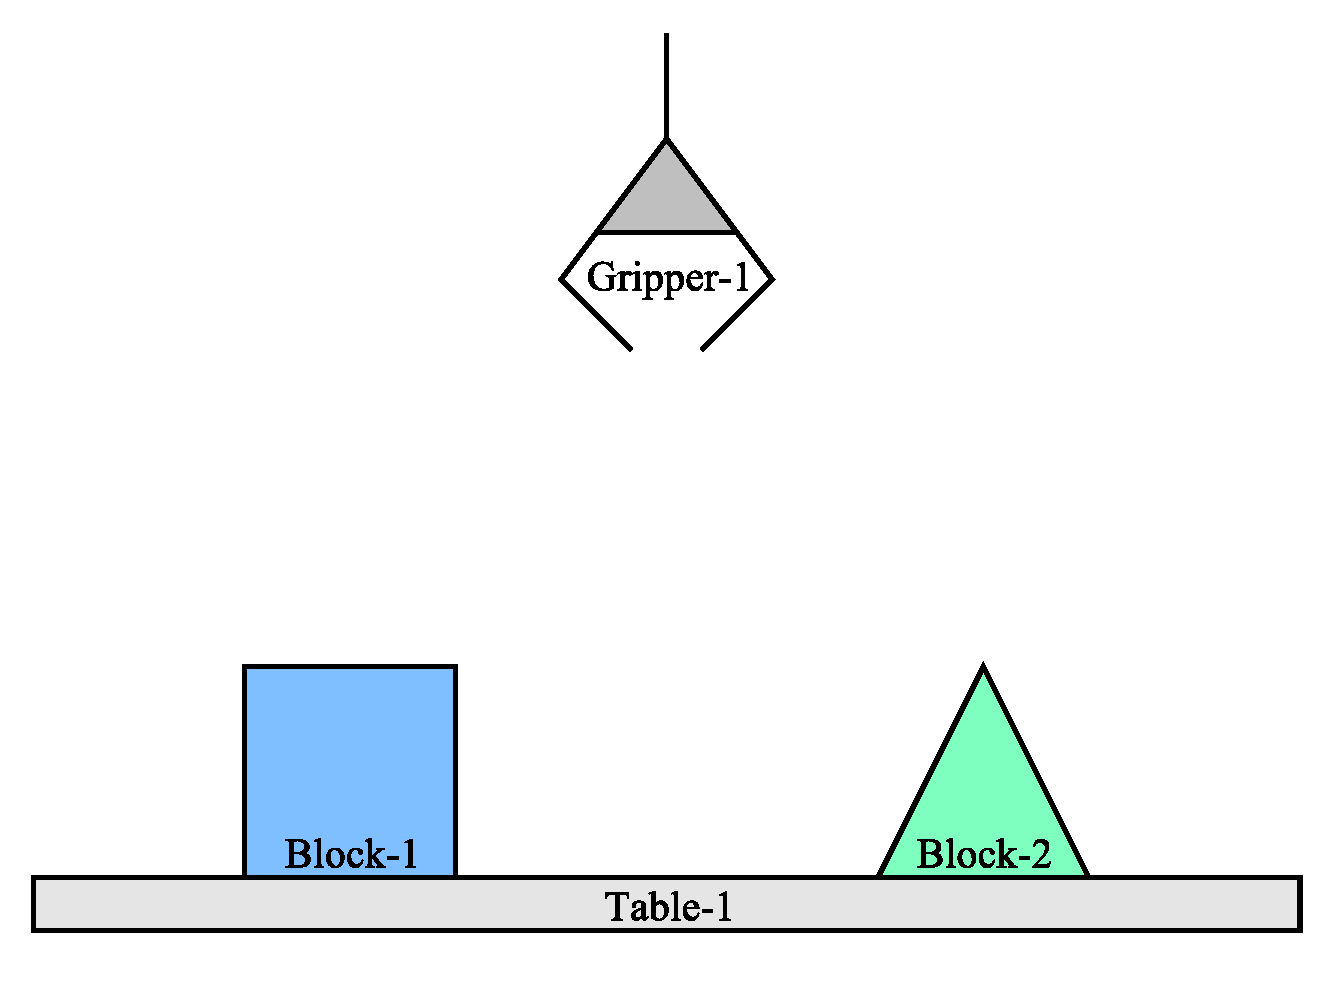
\includegraphics[width=8cm]{gfx/blocks_world_example-1}
\end{center}
\caption[An example problem domain.]{An example problem domain.}
\label{figure:an_example_problem_domain}
\end{figure}
\begin{figure}
\begin{center}
\begin{tabular}{p{4cm}p{4cm}}
1. 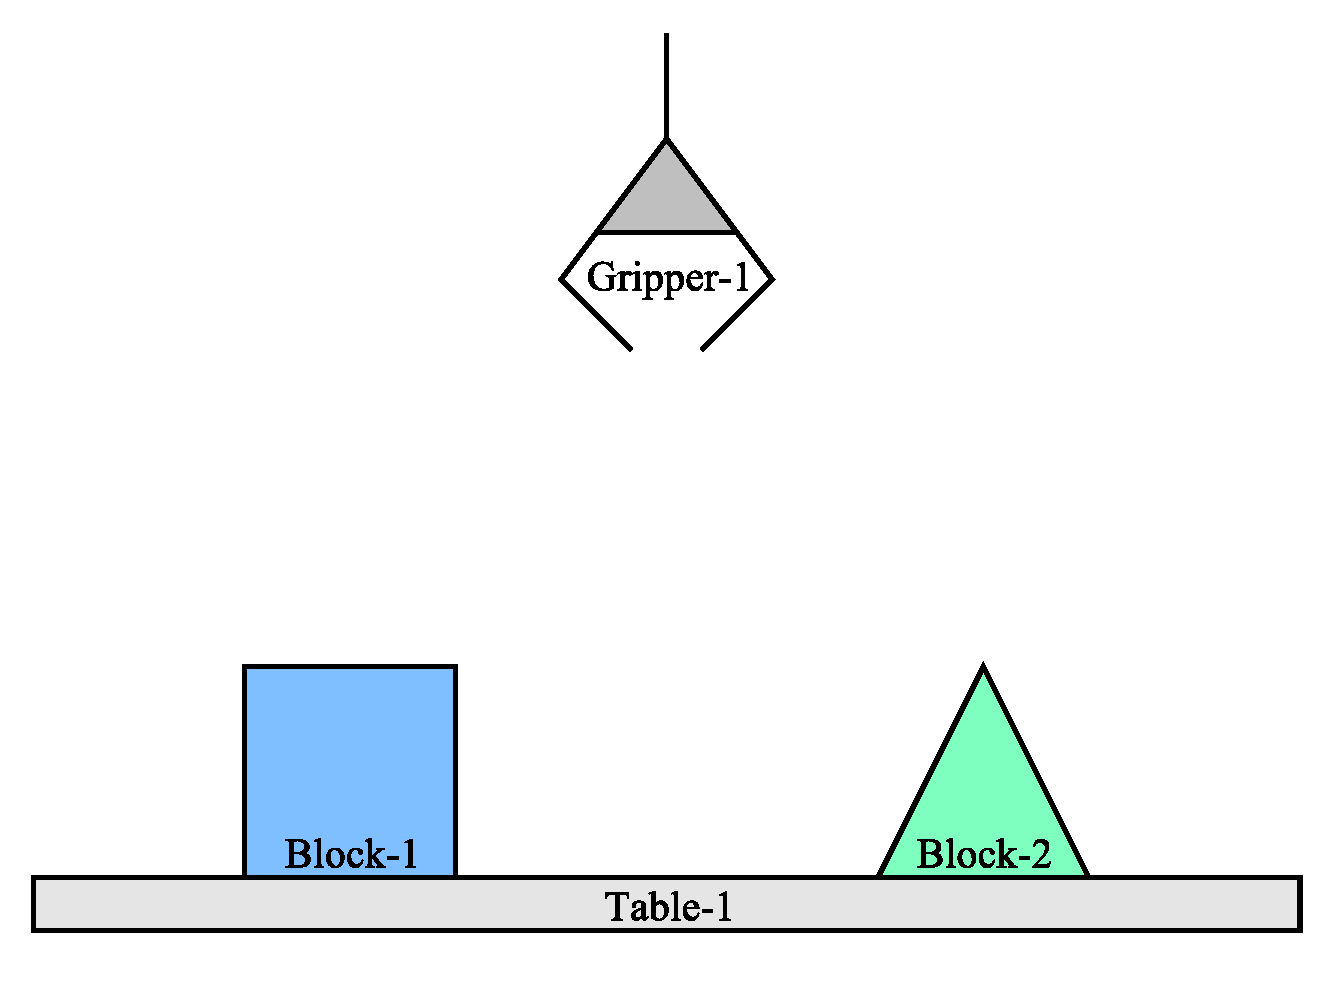
\includegraphics[width=5cm]{gfx/blocks_world_example-1}  & 2. 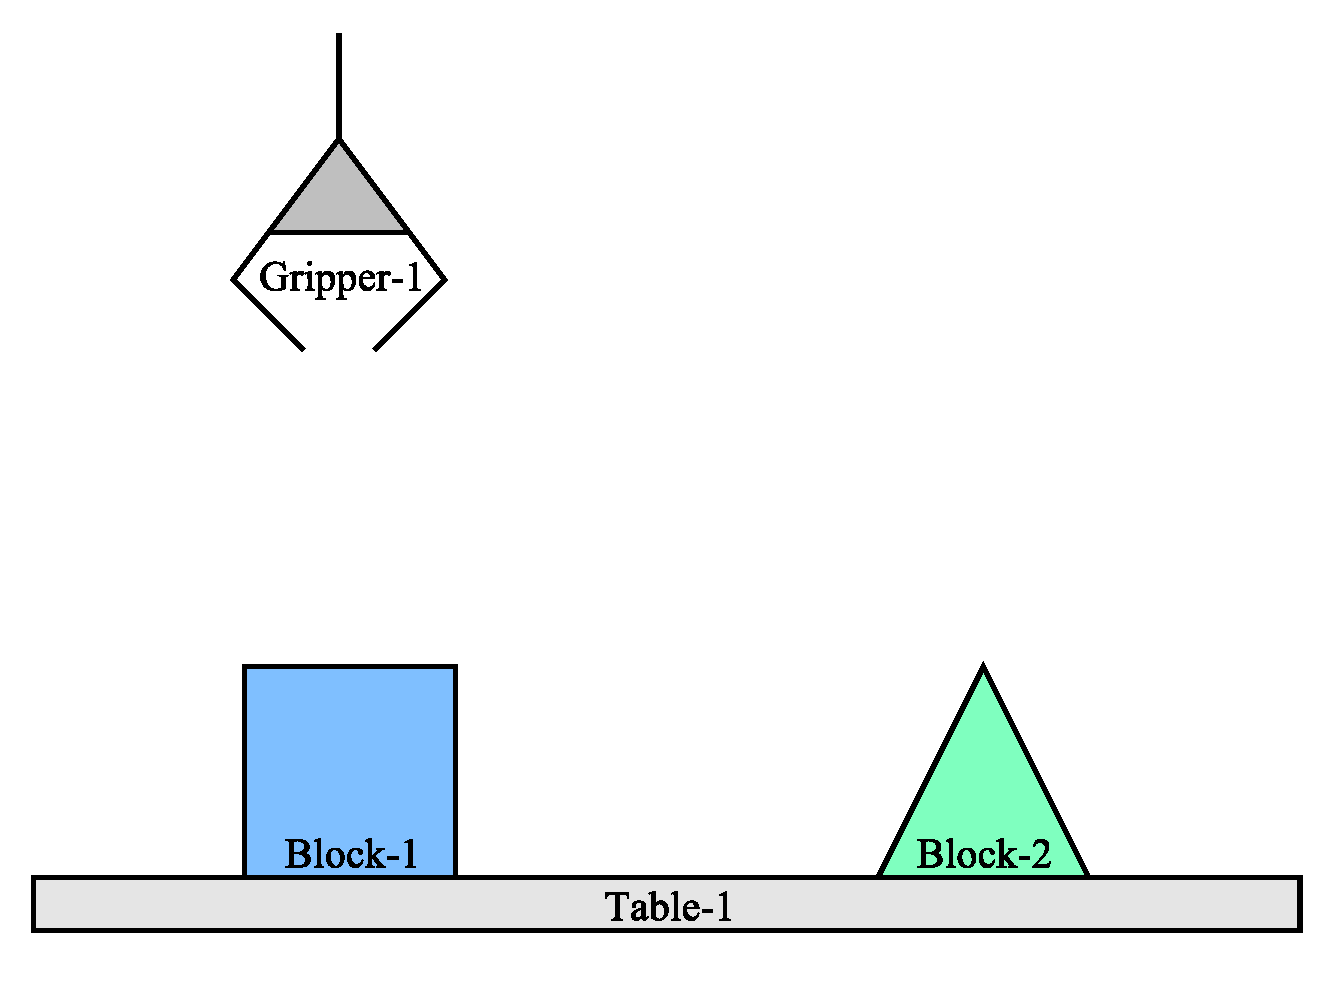
\includegraphics[width=5cm]{gfx/blocks_world_example-2} \\
3. 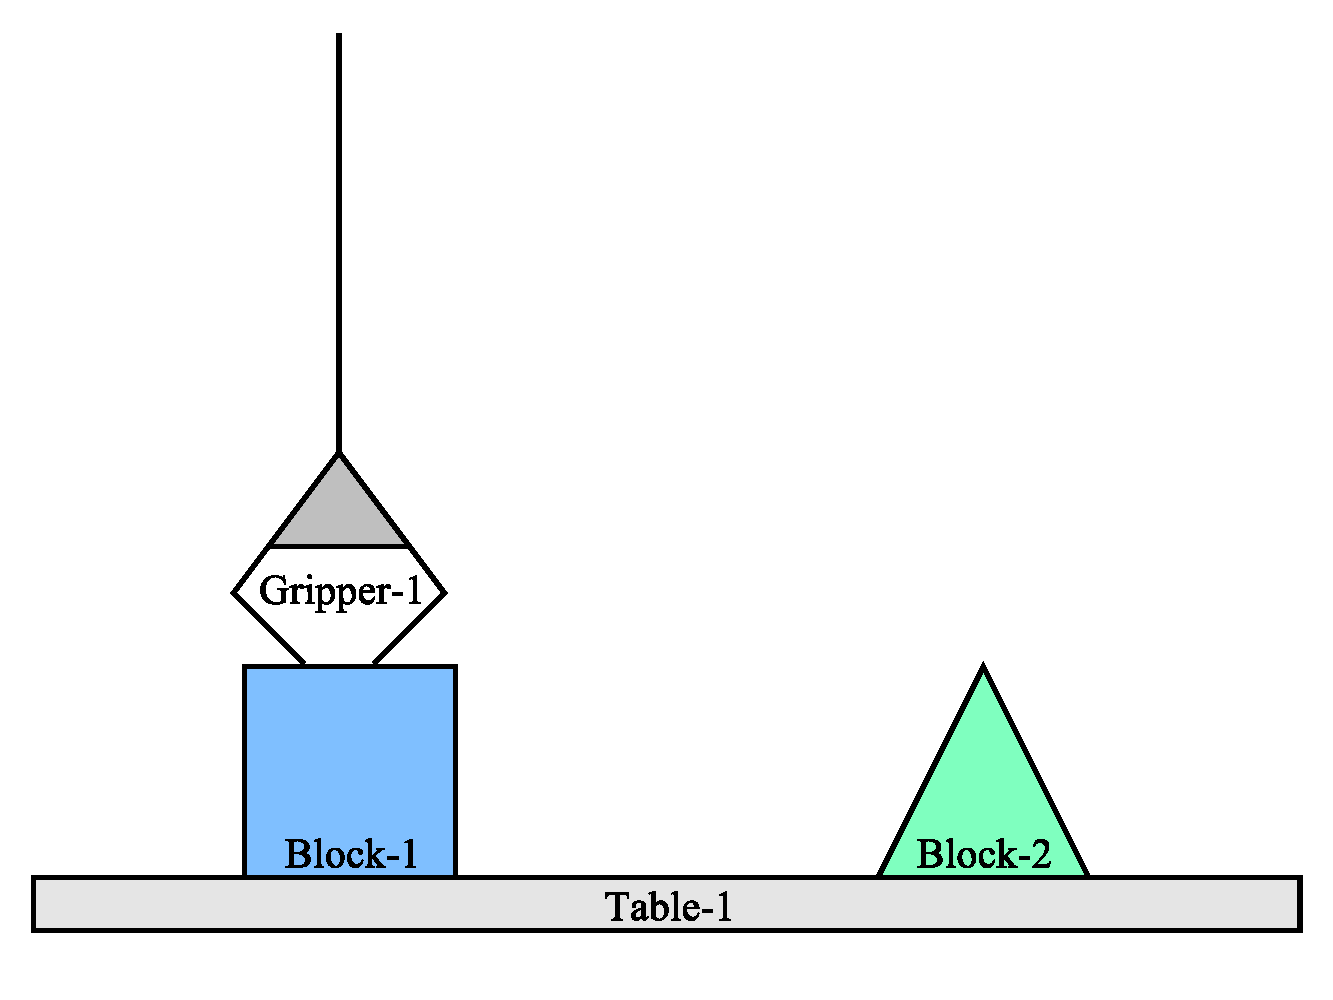
\includegraphics[width=5cm]{gfx/blocks_world_example-3}  & 4. 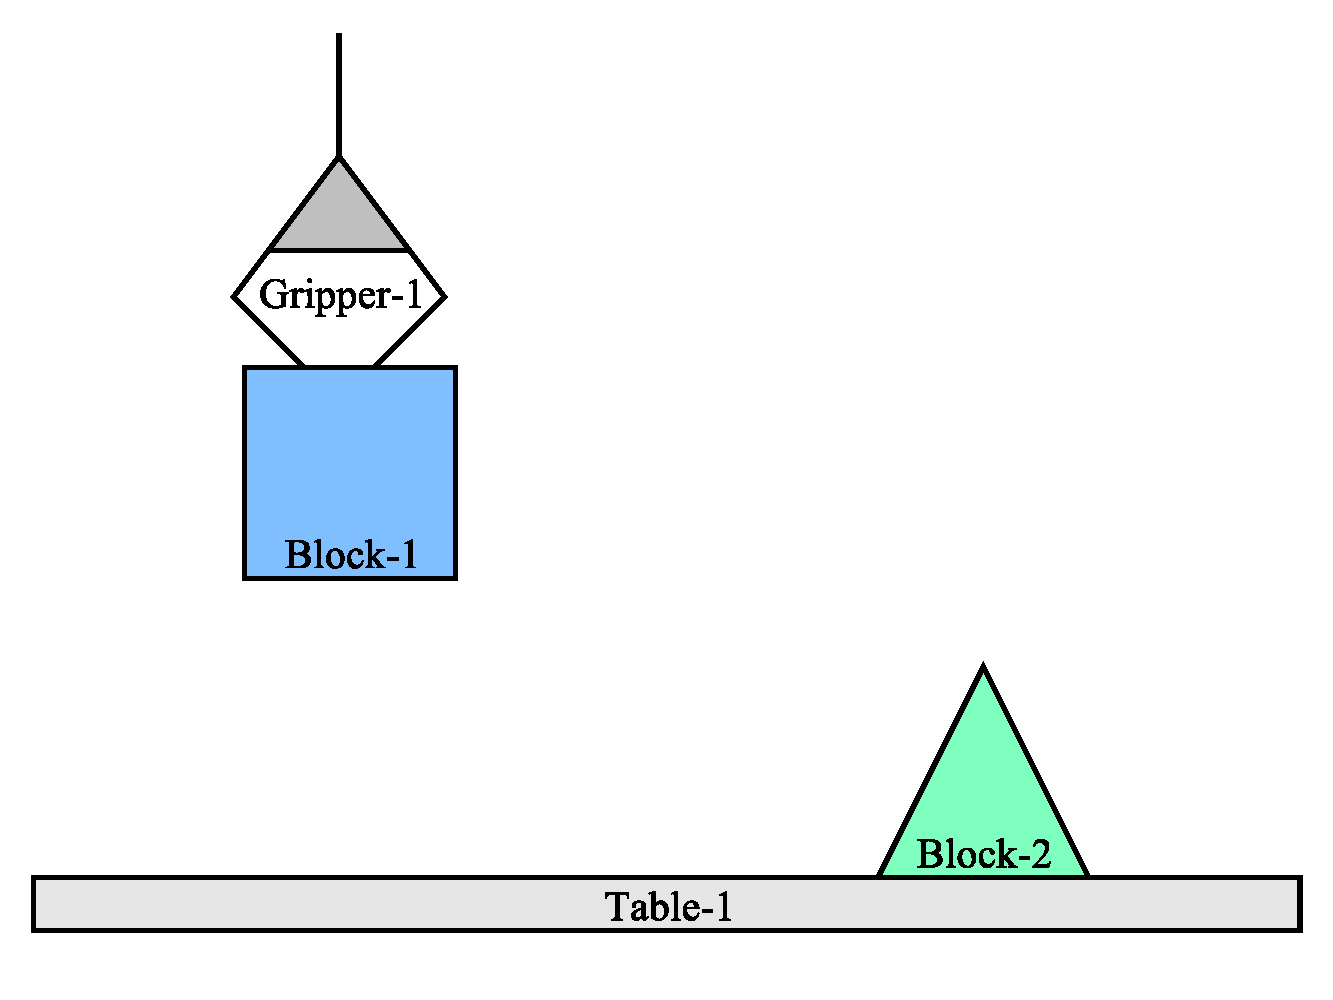
\includegraphics[width=5cm]{gfx/blocks_world_example-4} \\
5. 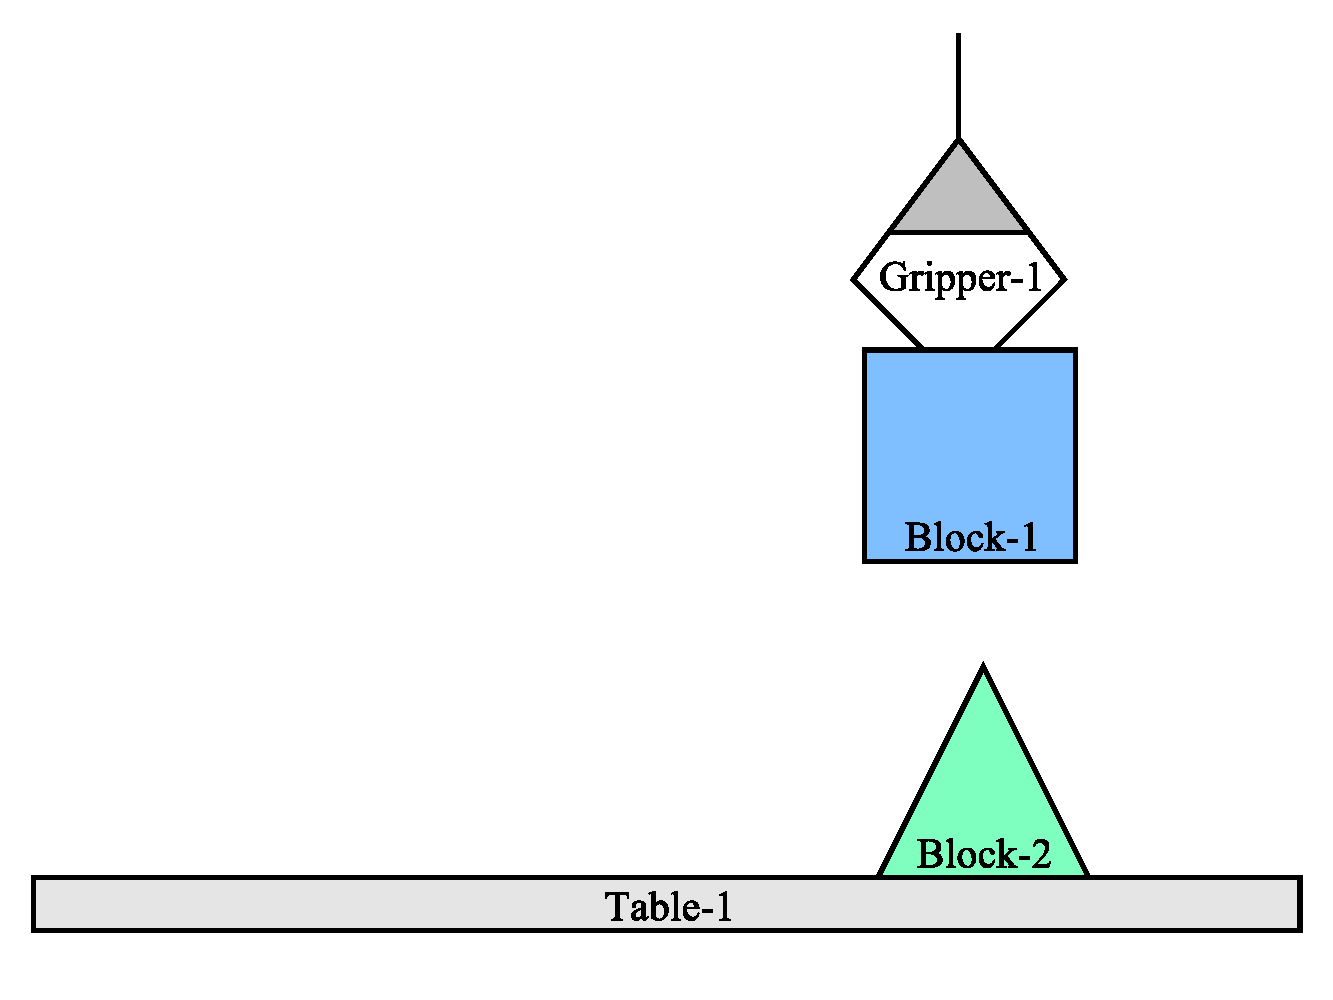
\includegraphics[width=5cm]{gfx/blocks_world_example-5}  & 6. 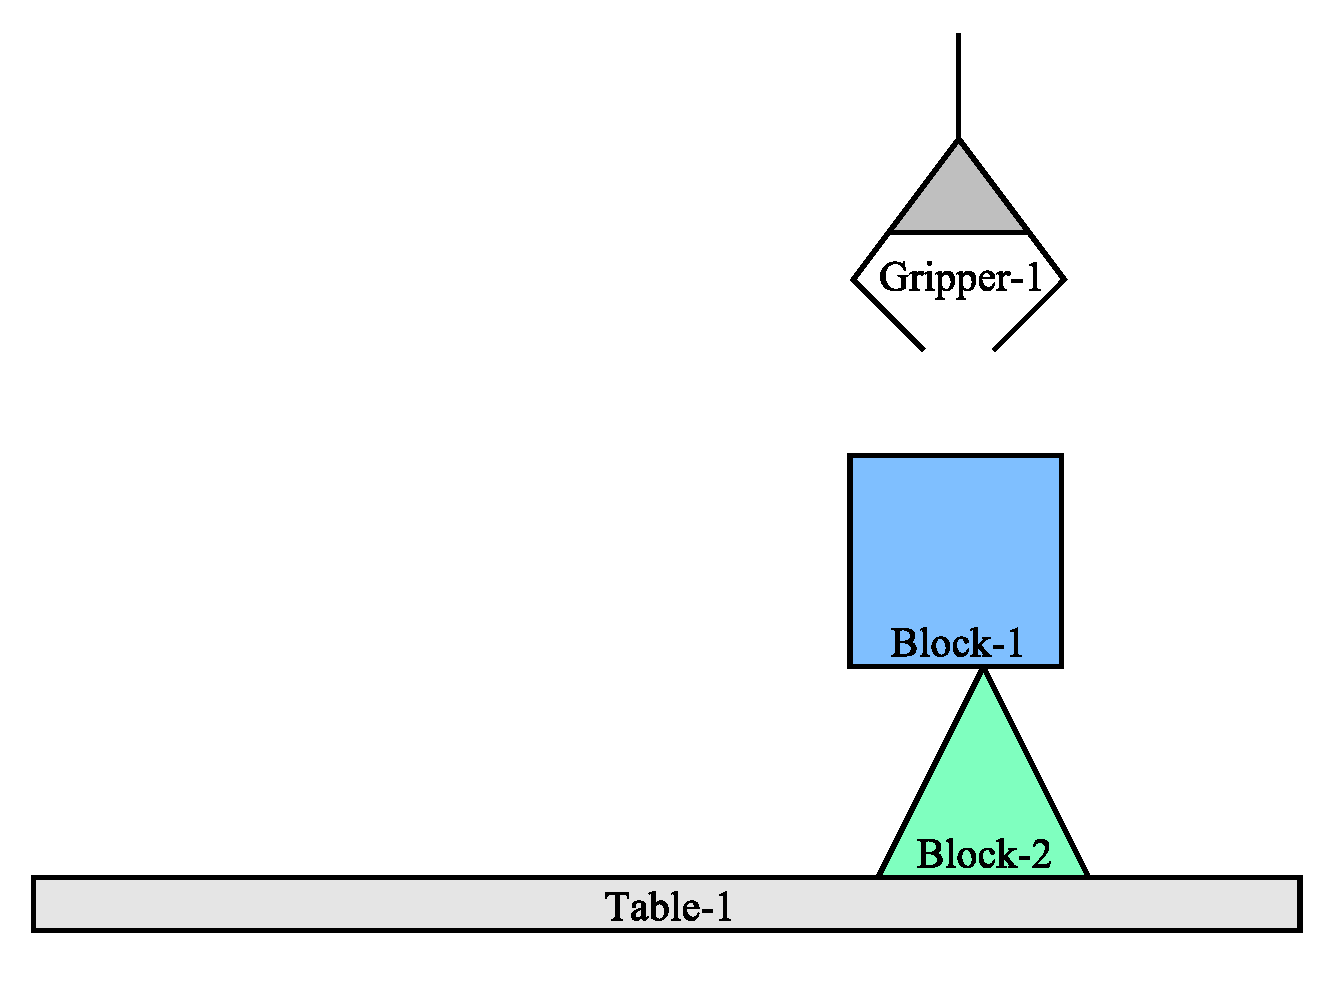
\includegraphics[width=5cm]{gfx/blocks_world_example-6} \\
7. 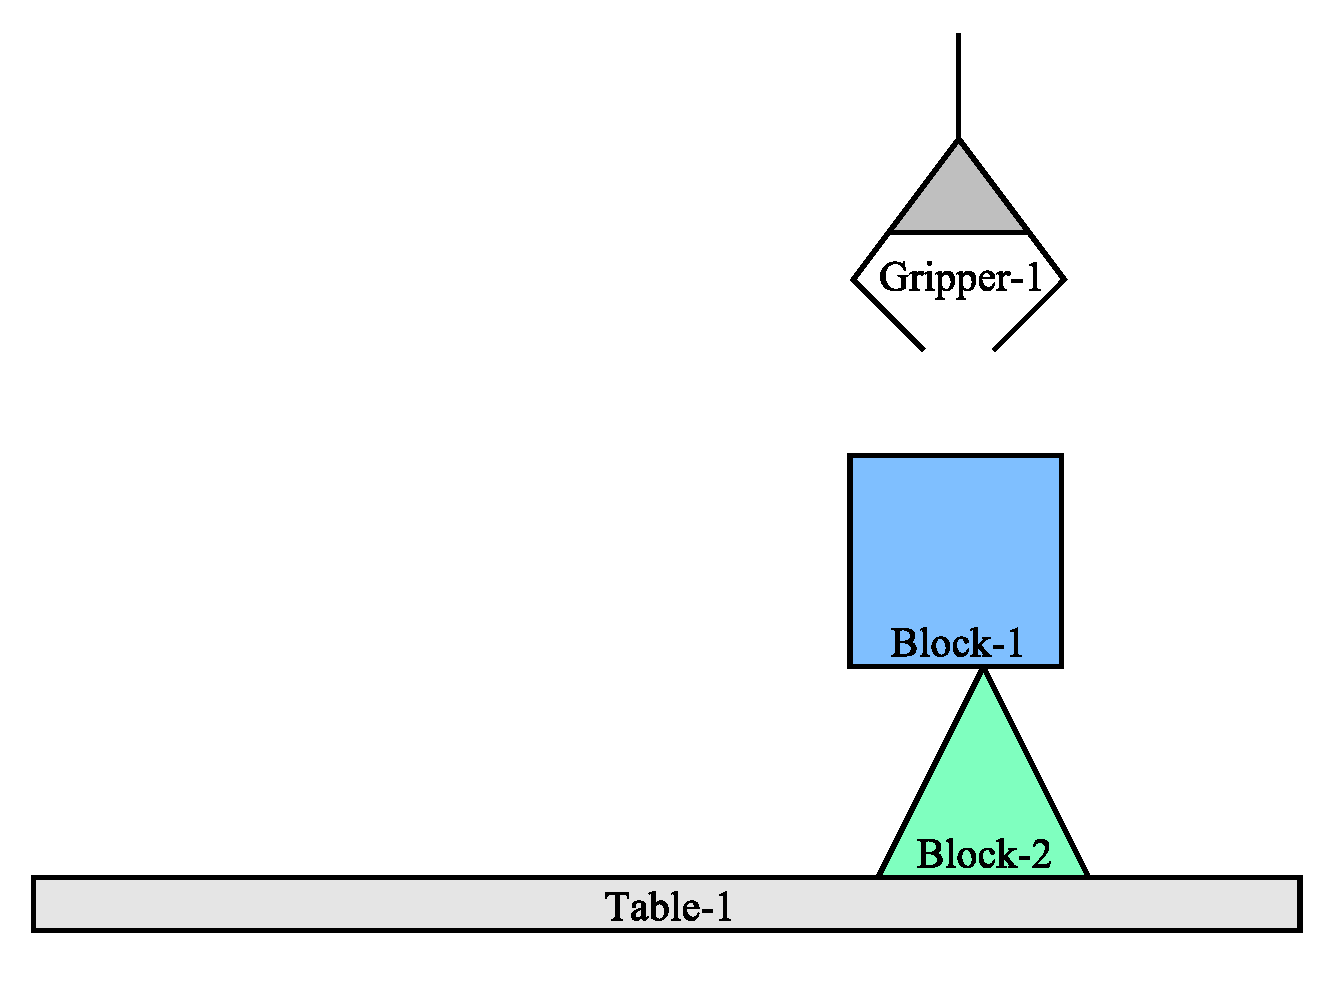
\includegraphics[width=5cm]{gfx/blocks_world_example-7}  & 8. 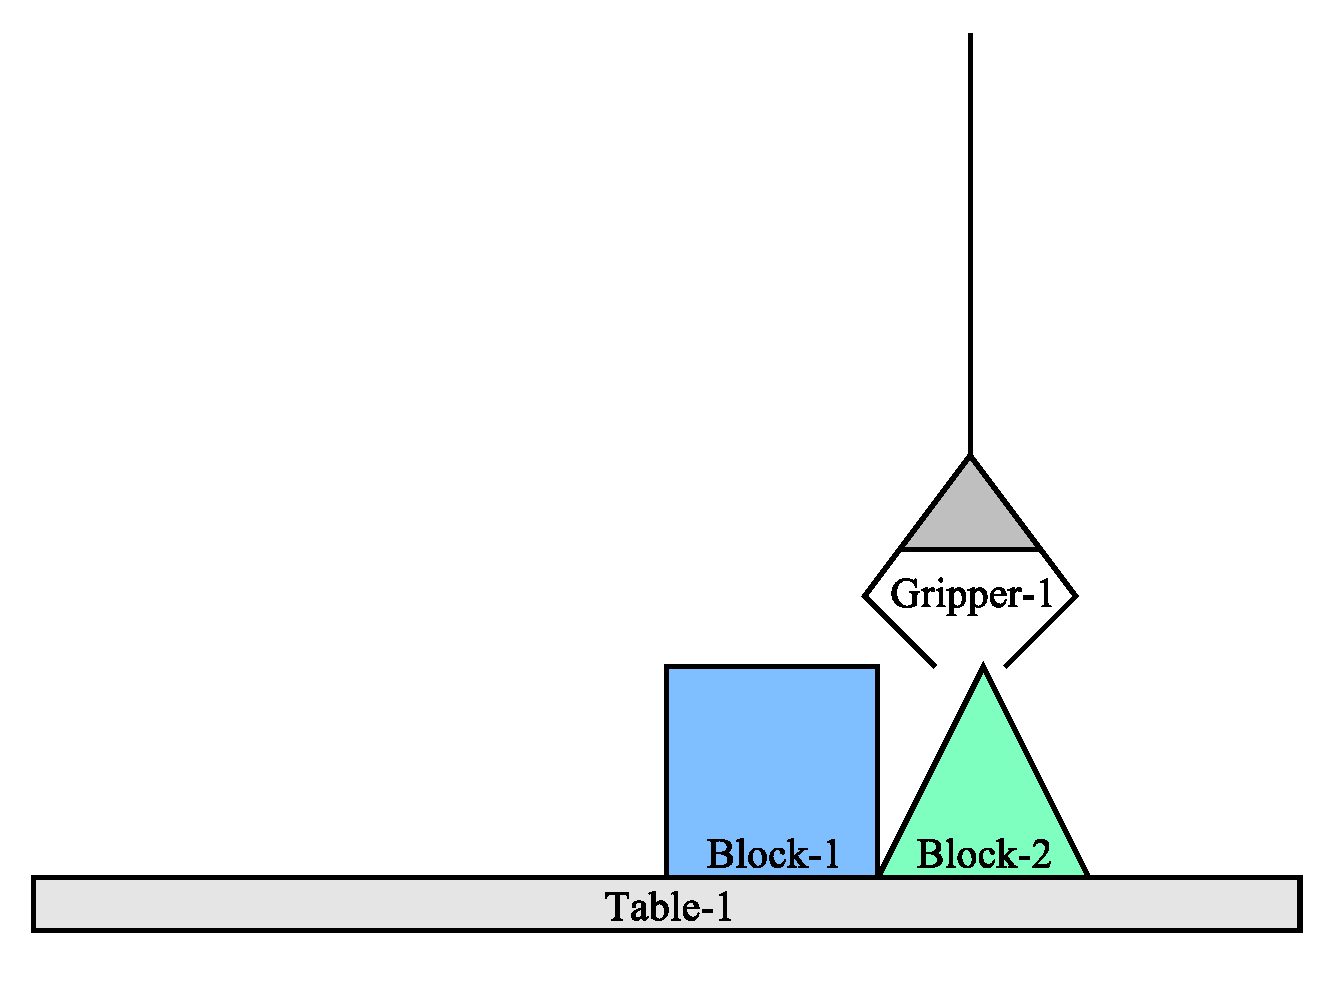
\includegraphics[width=5cm]{gfx/blocks_world_example-8}
\end{tabular}
\end{center}
\caption[An example of failing to accomplish a goal.]{An example of
  failing to accomplish the goal of creating a stack of two blocks.}
\label{figure:implemented_example_learning_storyboard}
\end{figure}


\section{The Physical Simulation}

The block building domain is implemented as a simulation based on
two-dimensional ridid-body physical laws, including floating point
numerical representations for object positions, velocities and
accellerations.  These numerical representations and the processes
that manipulate them are part of the physical layer of the model, but
in order to focus the efficiency of the procedural reflection, a much
simpler relational graph representation has been specifically
represented as semantic frame-based objects in a semantic
knowledge-base, referred to as the \emph{physical knowledge-base}.
For example, the semantic knowledge can be thought of as a list of the
following types of sentences:
\begin{itemize}
\item Block-1 is a block.
\item Block-2 is a block.
\item Table-1 is a table.
\item Gripper-1 is a gripper.
\item Block-1 has a blue color.
\item Block-1 has a cube shape.
\item Block-2 has a green color.
\item Block-2 has a pyramid shape.
\item Table-1 has a white color.
\item Gripper-1 has a black color.
\item Block-1 is on Table-1.
\item Block-2 is on Table-1.
\item Gripper-1 is above Table-1.
\item Block-1 is to the left of Gripper-1.
\item Block-2 is to the right of Gripper-1.
\end{itemize}
These sentences can be slightly rearranged to be thought of as
subject-verb-object triples as in the following list:
\begin{itemize}
\item Block-1 is-a block.
\item Block-2 is-a block.
\item Table-1 is-a table.
\item Gripper-1 is-a gripper.
\item Block-1 has-a-color blue.
\item Block-1 has-a-shape cube.
\item Block-2 has-a-color green.
\item Block-2 has-a-shape pyramid.
\item Table-1 has-a-color white.
\item Gripper-1 has-a-color black.
\item Block-1 is-on Table-1.
\item Block-2 is-on Table-1.
\item Gripper-1 is-above Table-1.
\item Block-1 is-to-the-left-of Gripper-1.
\item Block-2 is-to-the-right-of Gripper-1.
\end{itemize}
The physical simulation maintains a list of these simple
subject-verb-object sentences in its internal state.  The actual
internal lisp-like representation of the physical simulation is shown
in \autoref{table:internal_lisp_like_physical_representation}.
\begin{table}
\begin{center}
{\fbox{
\begin{tabular}{l}
 {\tt{[Block-1 left-of Gripper-1]}} \\
 {\tt{[Block-1 on Table-1]}} \\
 {\tt{[Block-1 shape cube]}} \\
 {\tt{[Block-1 color blue]}} \\
 {\tt{[Block-1 is-a block]}} \\
 {\tt{[Block-2 right-of Gripper-1]}} \\
 {\tt{[Block-2 on Table-1]}} \\
 {\tt{[Block-2 shape pyramid]}} \\
 {\tt{[Block-2 color green]}} \\
 {\tt{[Block-2 is-a block]}} \\
 {\tt{[Table-1 left-of Gripper-1]}} \\
 {\tt{[Table-1 shape cube]}} \\
 {\tt{[Table-1 color white]}} \\
 {\tt{[Table-1 is-a table]}} \\
 {\tt{[Gripper-1 is-holding []]}} \\
 {\tt{[Gripper-1 color black]}} \\
 {\tt{[Gripper-1 is-a gripper]}} \\
 {\tt{[Gripper-1 movement\_command stop]}} \\
 {\tt{[Gripper-1 is me]}}
\end{tabular}
}}
\end{center}
\caption[Internal representation for physical simulation.]{Internal representation for physical simulation.}
\label{table:internal_lisp_like_physical_representation}
\end{table}
{\mbox{\autoref{figure:implemented_physical_knowledge}}} shows the
physical knowledge-base that is reconstructed from these reflective
change events.
\begin{sidewaysfigure}
\begin{center}
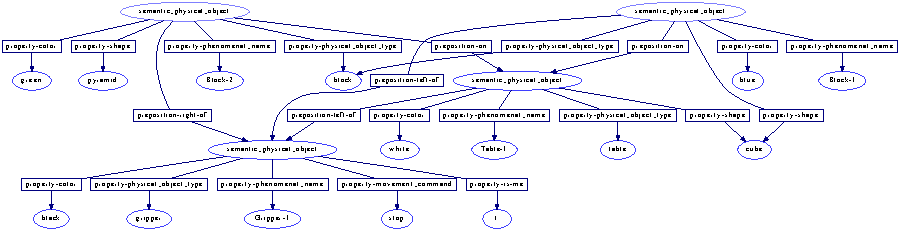
\includegraphics[width=24cm]{gfx/implemented_physical_knowledge}
\end{center}
\hspace{4cm}\parbox{15cm}{\caption[The physical knowledge-base.]{The
    physical
    knowledge-base.}\label{figure:implemented_physical_knowledge}}
\end{sidewaysfigure}

\section{Procedurally Reflective Event Stream}



\section{Abstraction}



\section{An Example Storyboard}

{\mbox{\autoref{figure:implemented_example_learning_storyboard}}}
shows a storyboard of the implemented example of second-order
learning.
\begin{figure}
\begin{center}
\begin{tabular}{p{4cm}p{4cm}p{4cm}}
1. 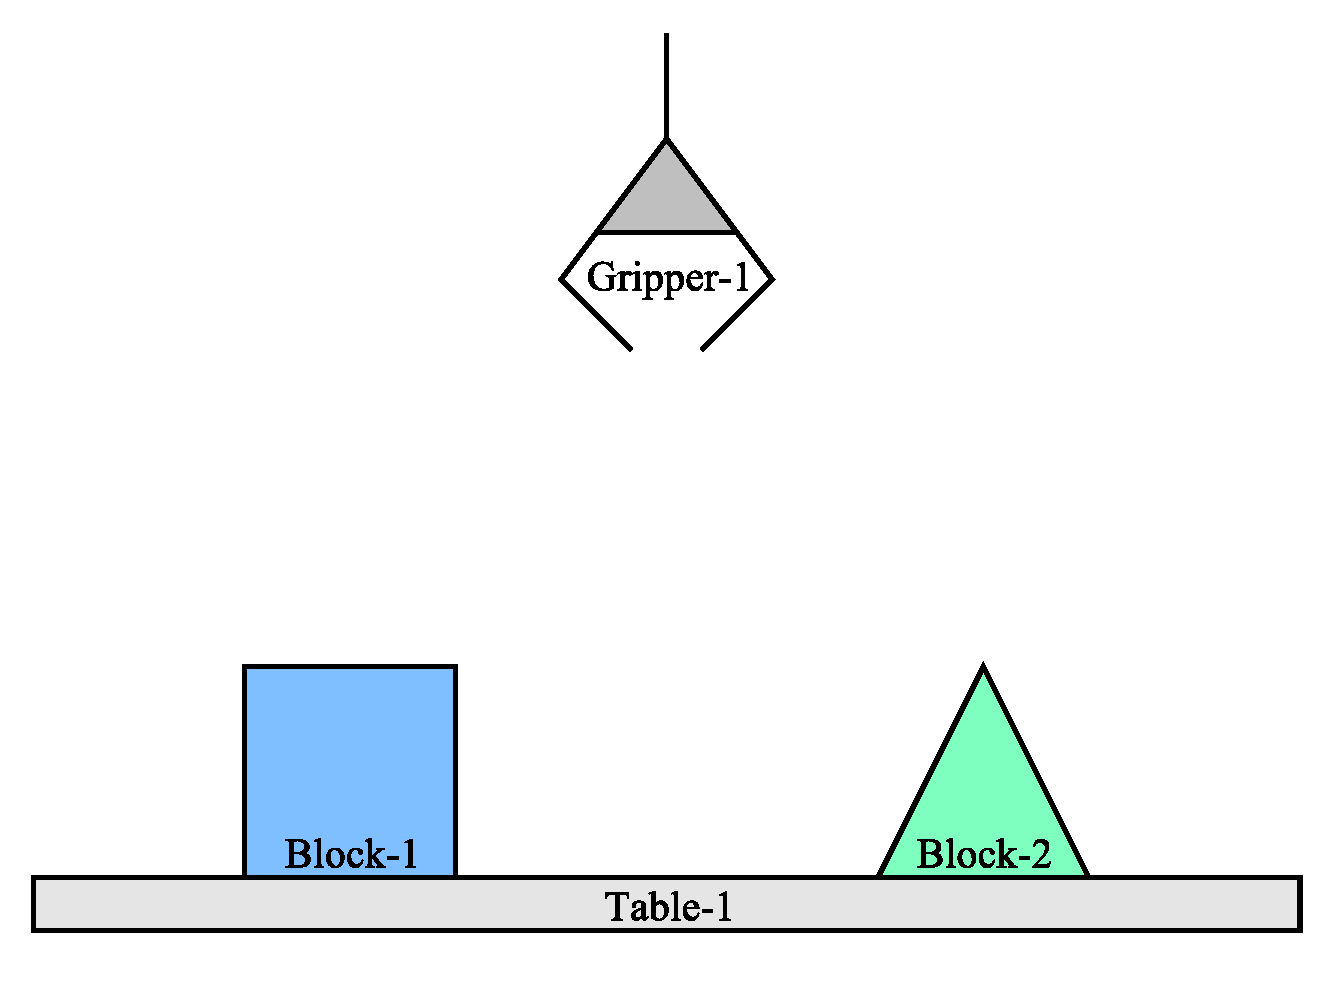
\includegraphics[width=4cm]{gfx/blocks_world_example-1}  & 2. 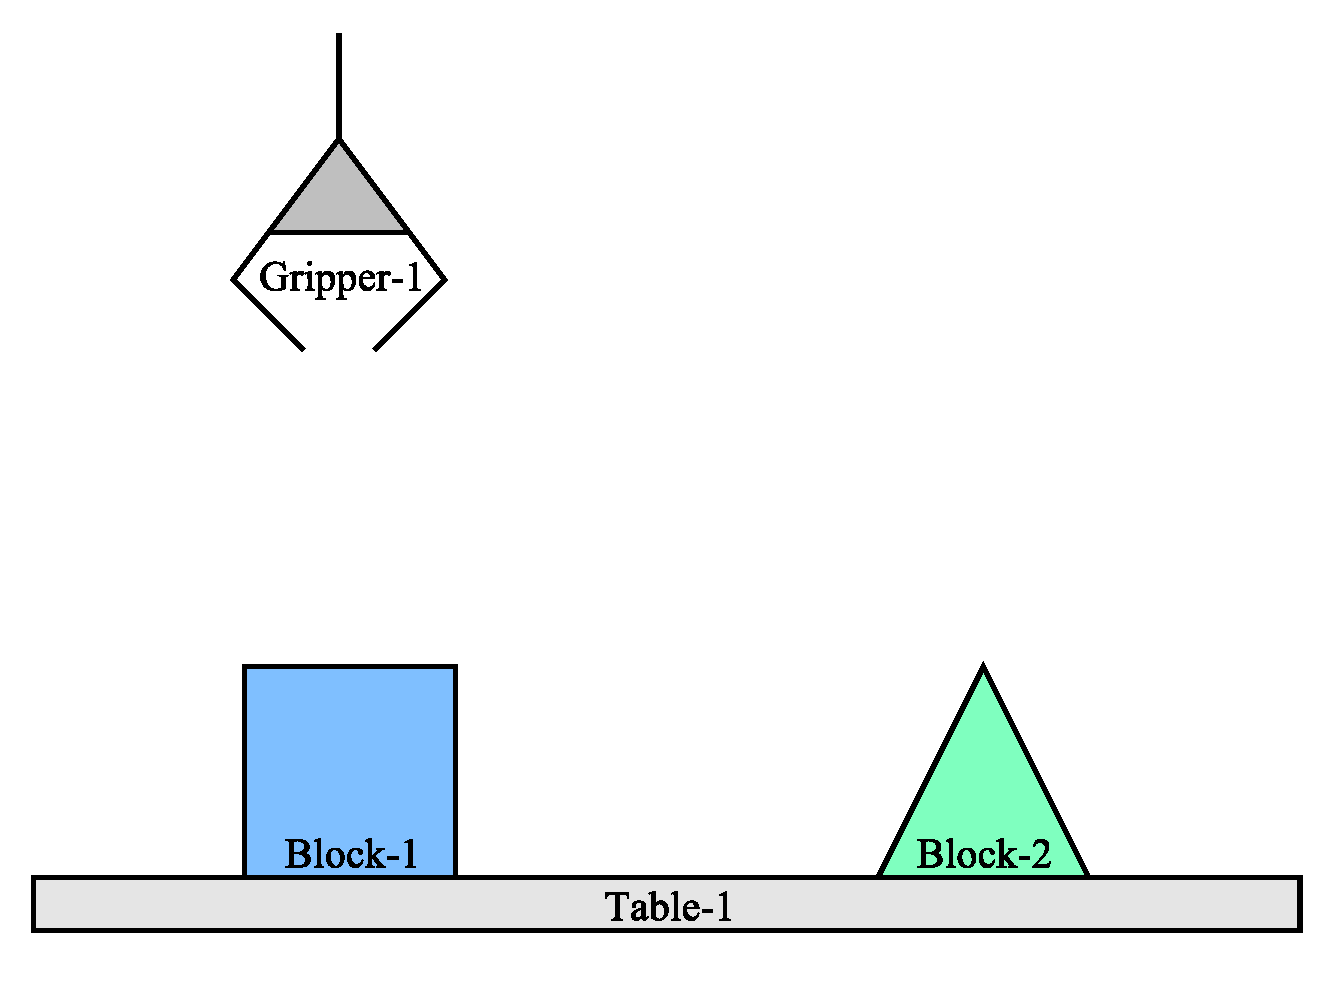
\includegraphics[width=4cm]{gfx/blocks_world_example-2}  & 3. 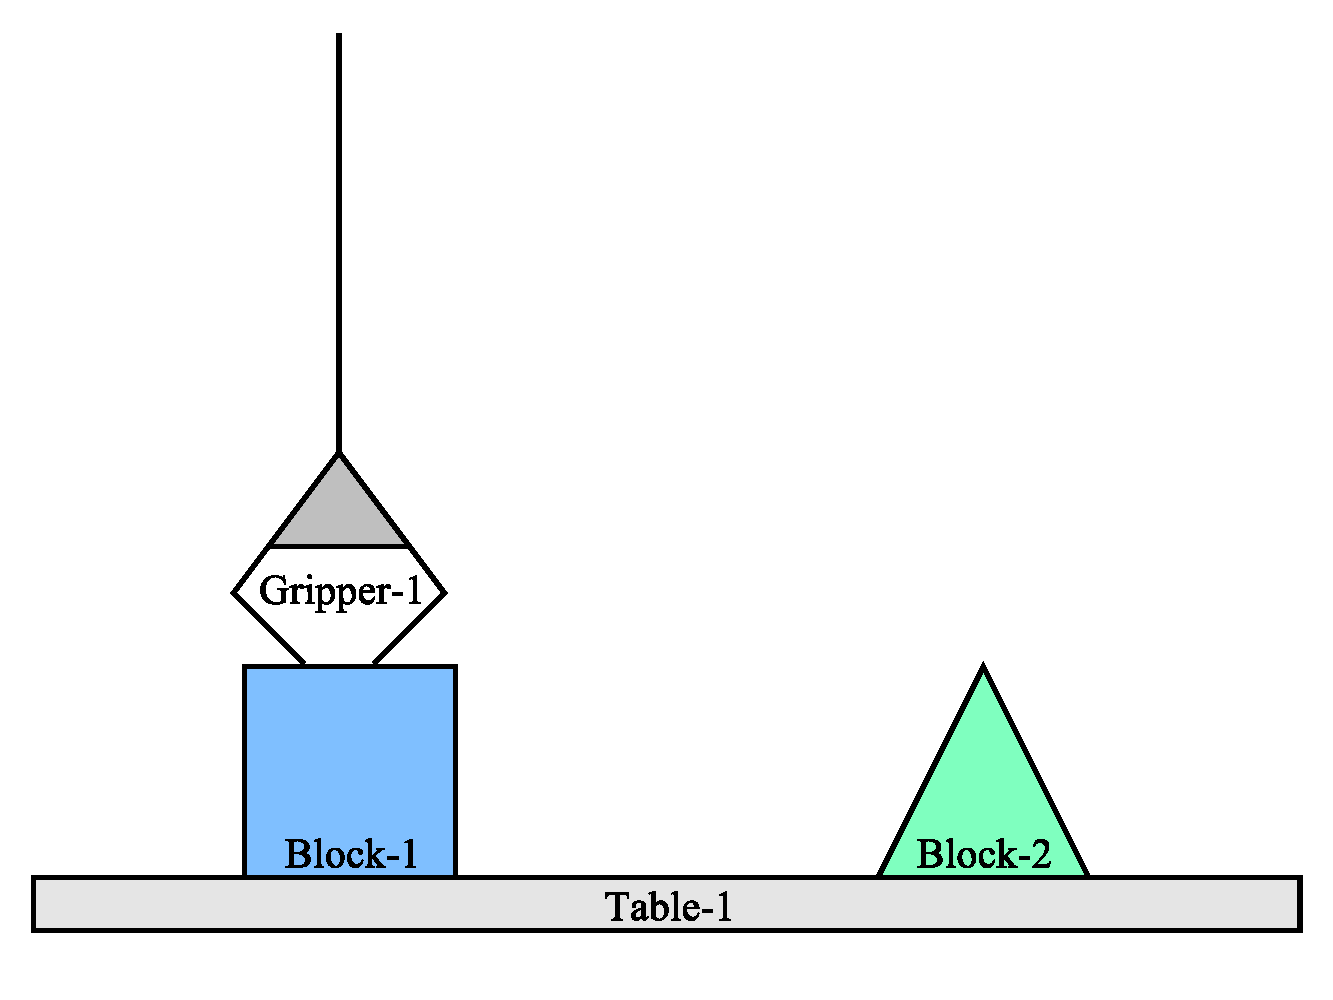
\includegraphics[width=4cm]{gfx/blocks_world_example-3} \\
4. 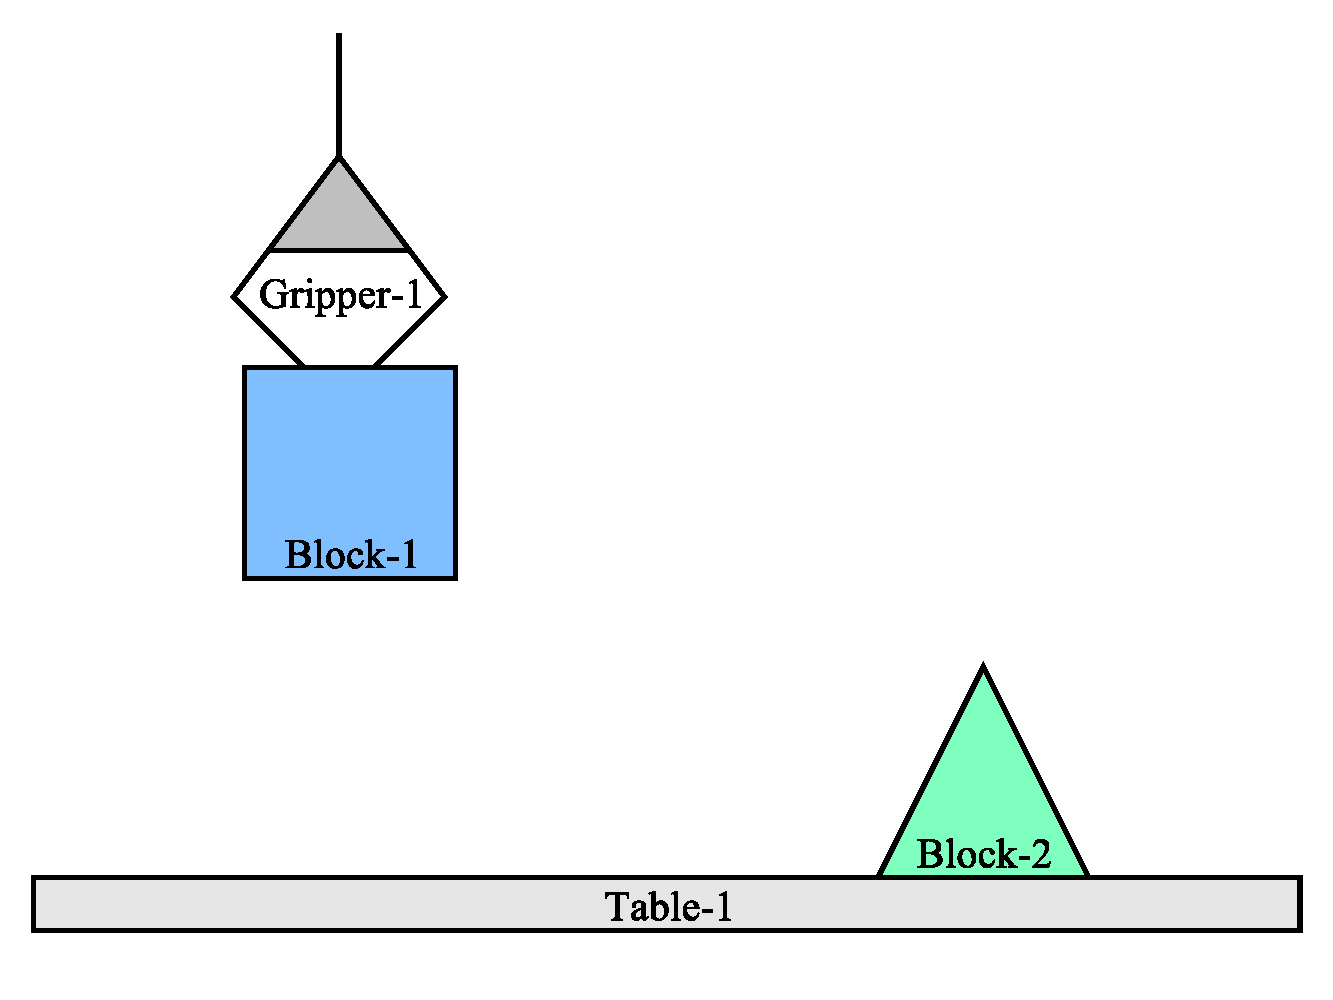
\includegraphics[width=4cm]{gfx/blocks_world_example-4}  & 5. 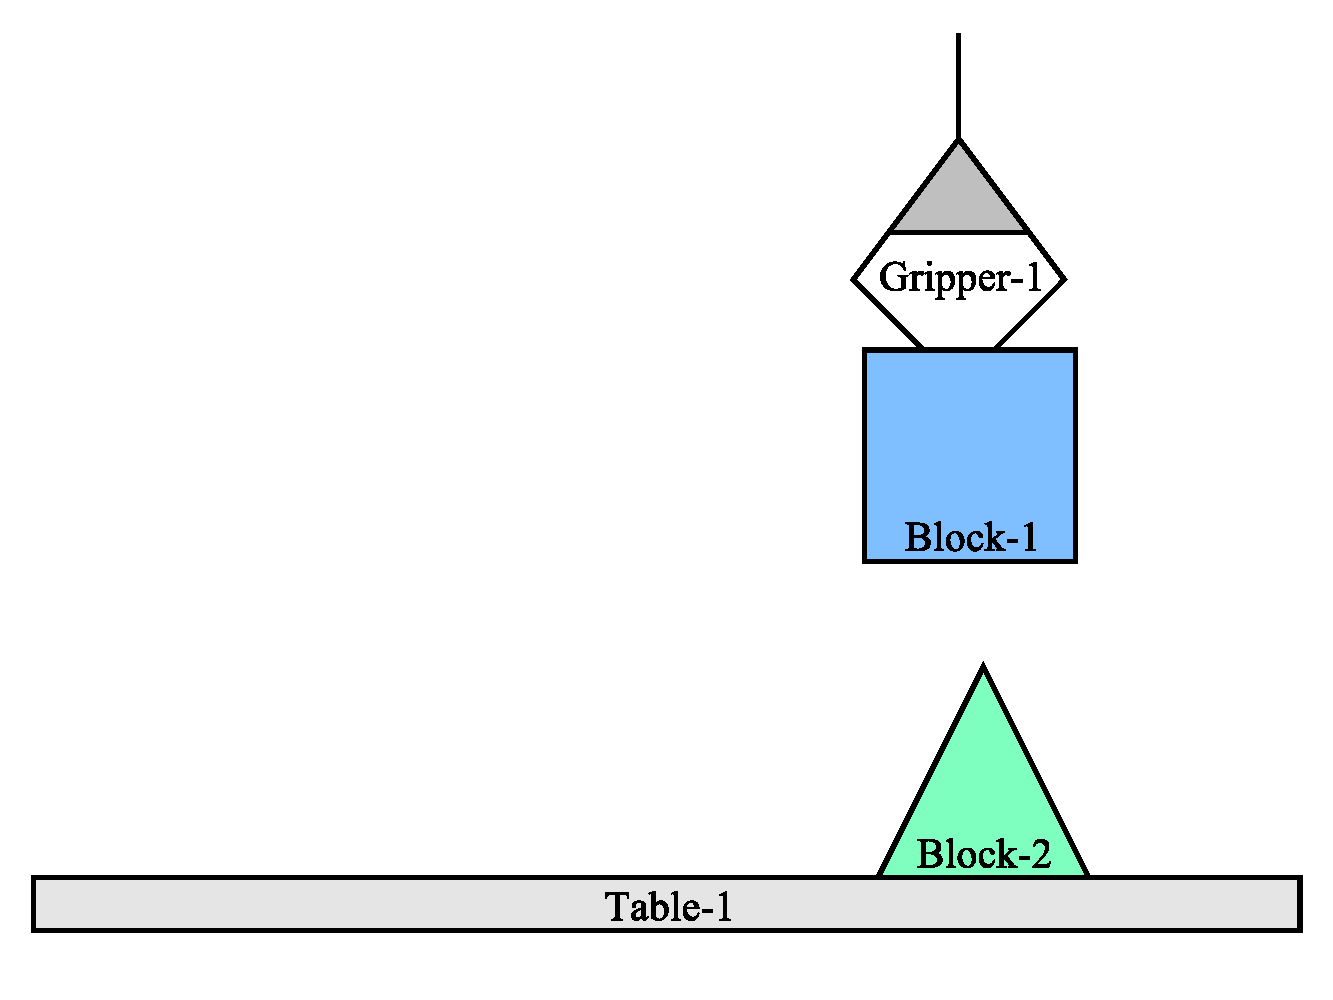
\includegraphics[width=4cm]{gfx/blocks_world_example-5}  & 6. 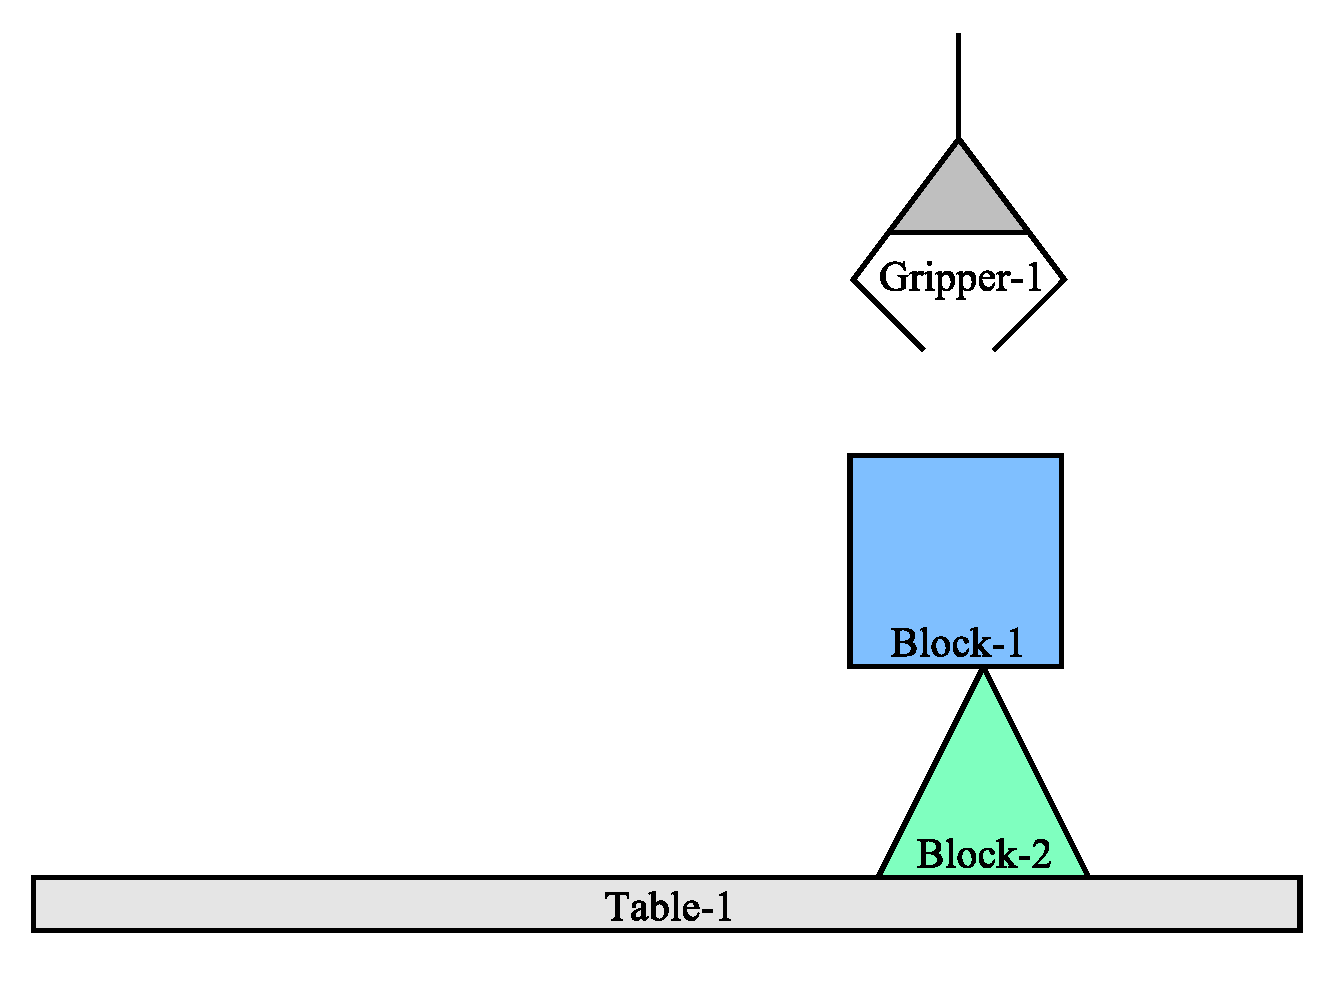
\includegraphics[width=4cm]{gfx/blocks_world_example-6} \\
7. 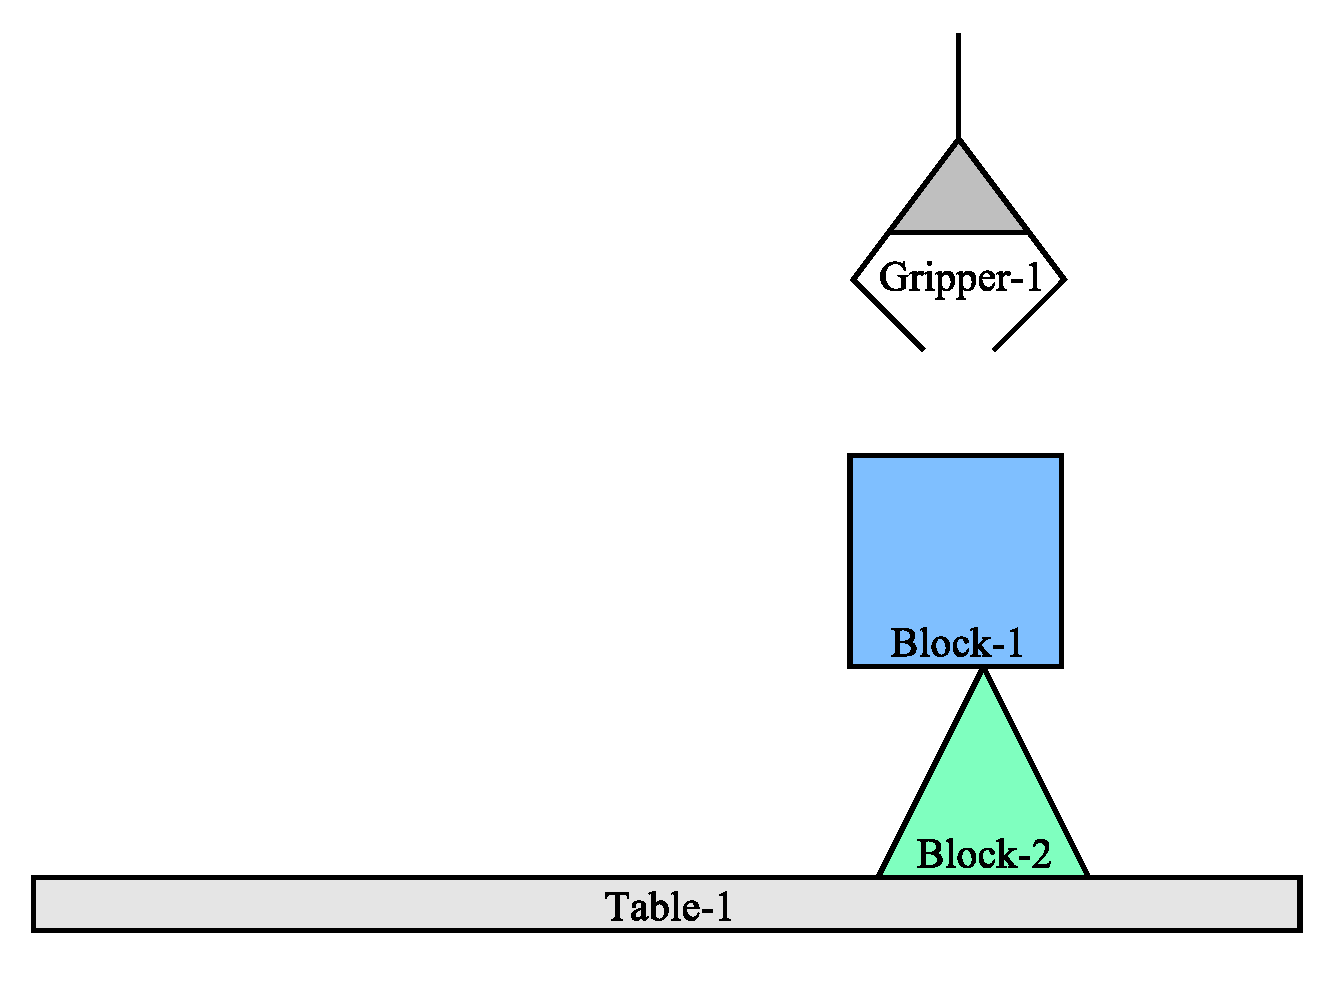
\includegraphics[width=4cm]{gfx/blocks_world_example-7}  & 8. 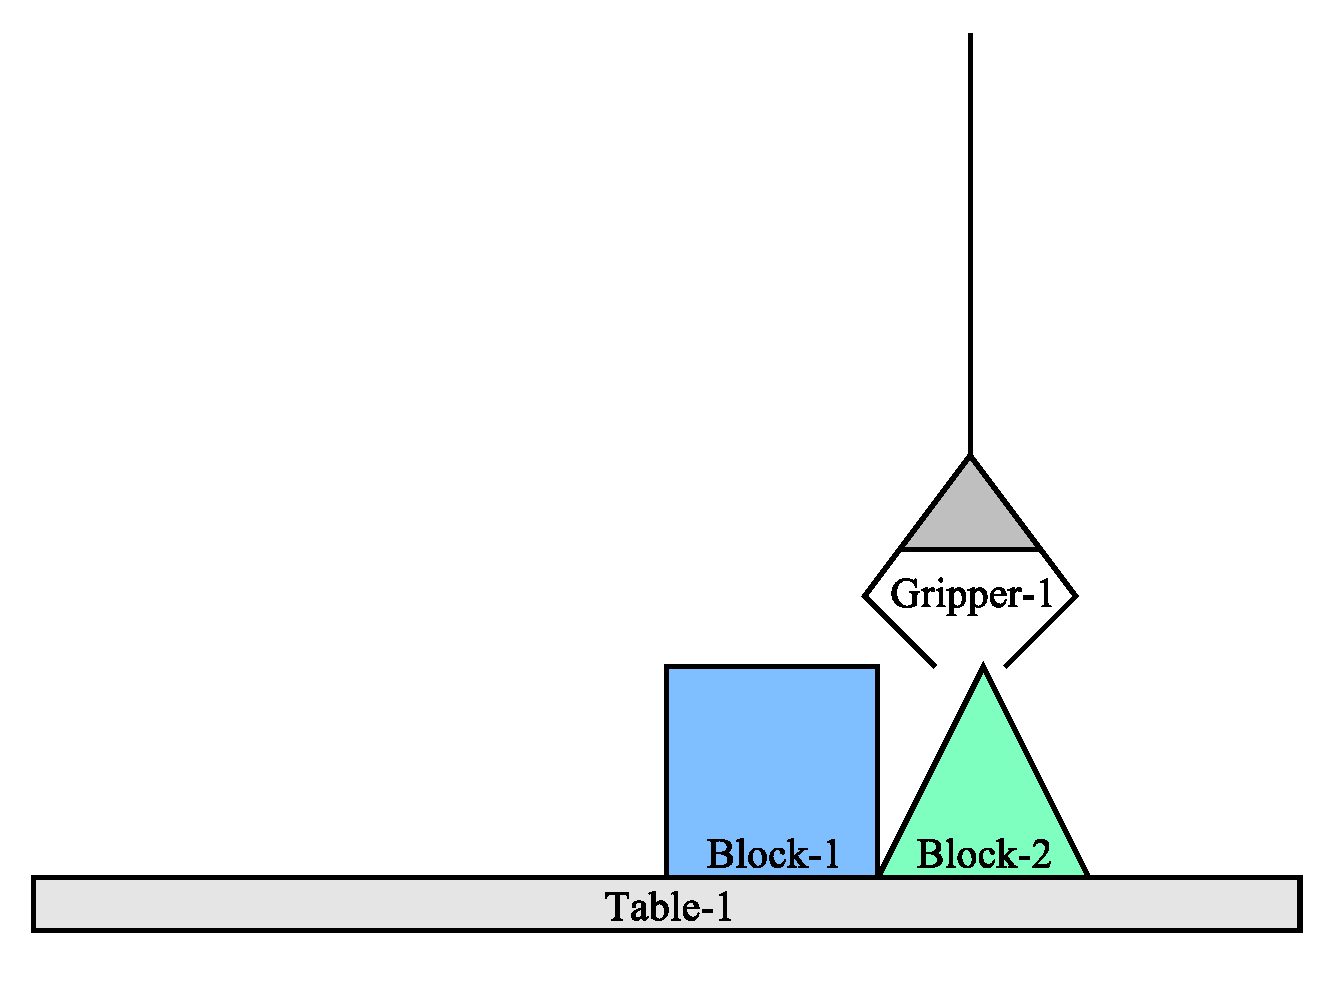
\includegraphics[width=4cm]{gfx/blocks_world_example-8}  & 9. 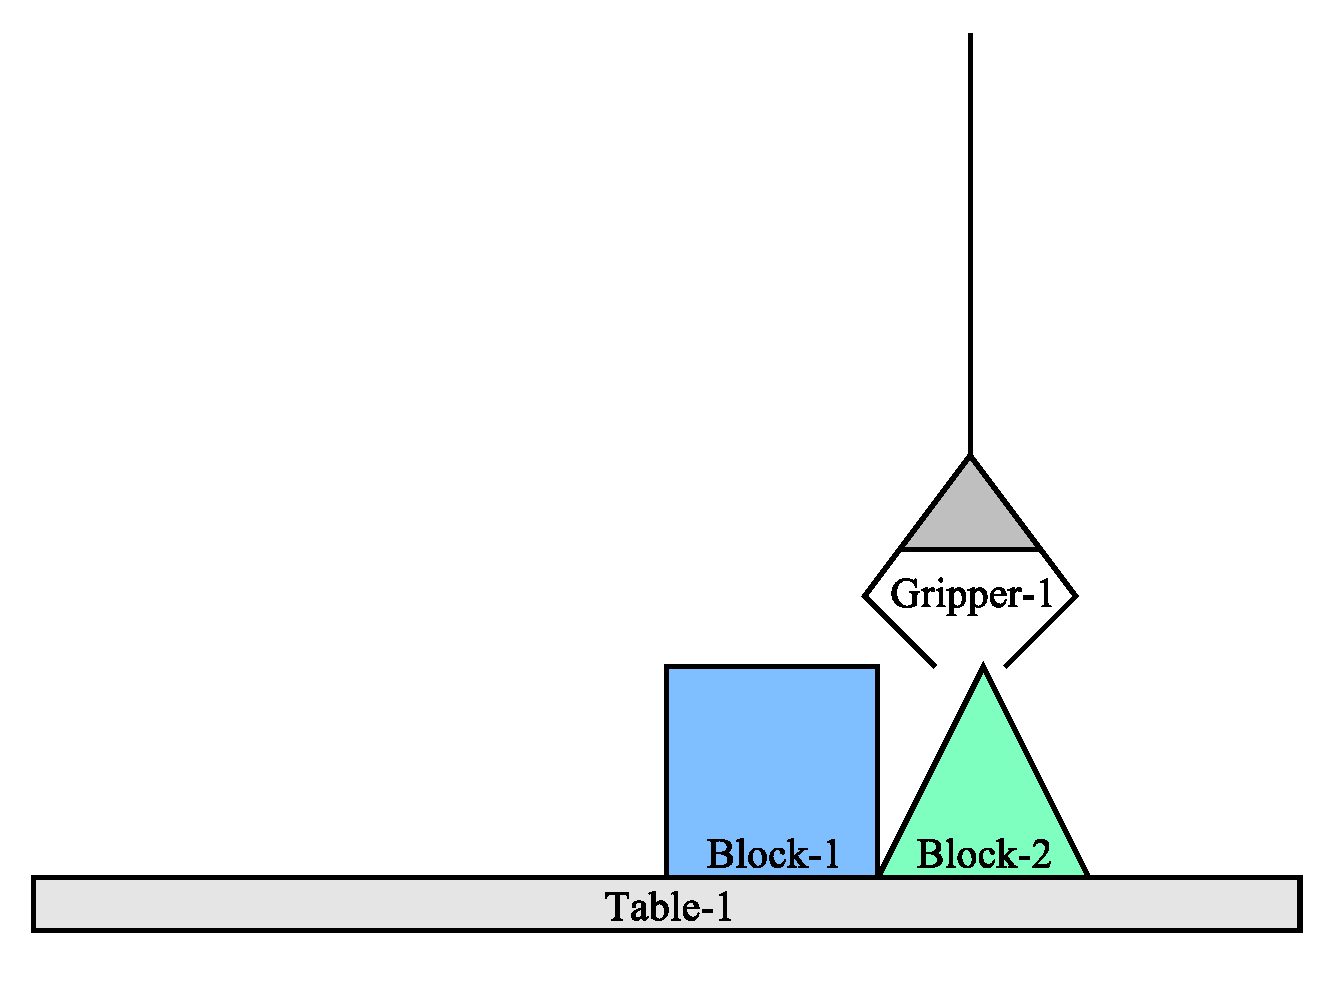
\includegraphics[width=4cm]{gfx/blocks_world_example-9} \\
10. 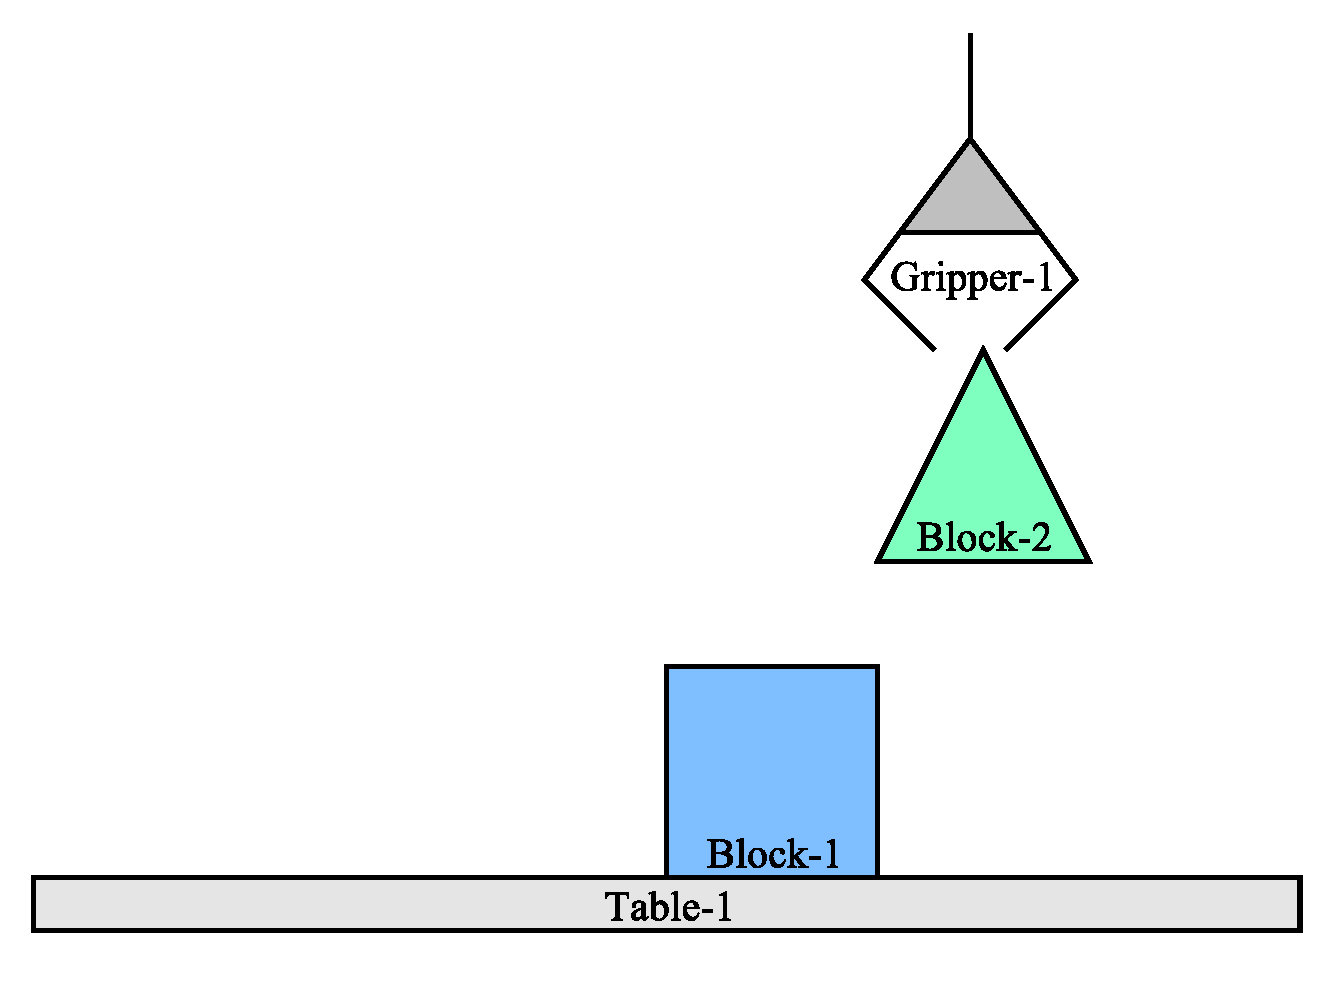
\includegraphics[width=4cm]{gfx/blocks_world_example-10} & 11. 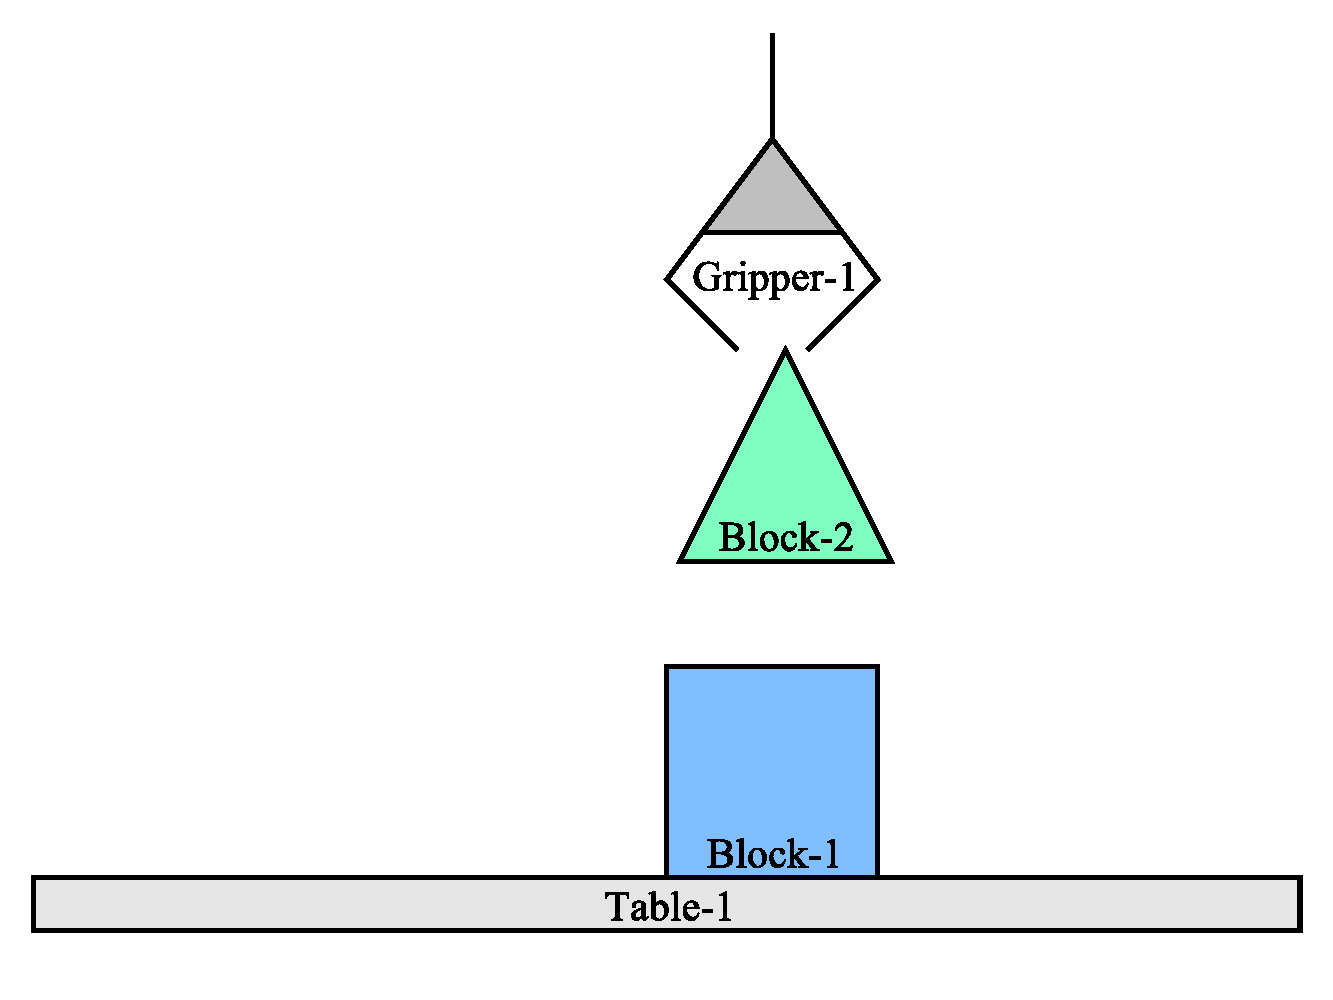
\includegraphics[width=4cm]{gfx/blocks_world_example-11} & 12. 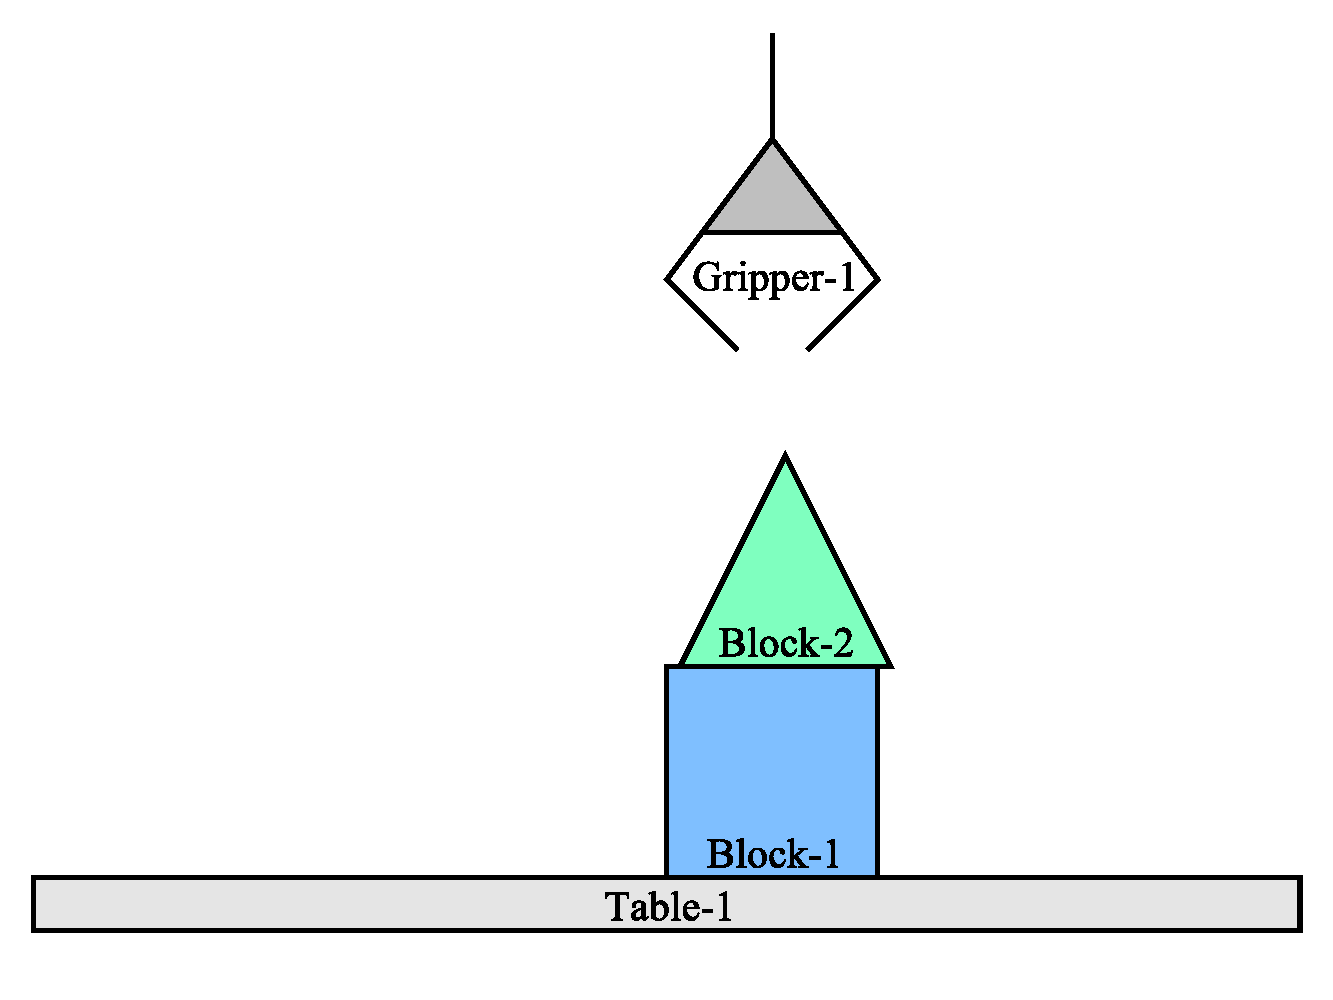
\includegraphics[width=4cm]{gfx/blocks_world_example-12}
\end{tabular}
\end{center}
\caption[A storyboard of the implemented example of second-order
  learning.]{A storyboarded example of second-order learning, where
  the goal is to create a stack of two blocks.  (1) A plan that is
  hypothesized to stack the square block on top of the triangular
  block is executed.  (2--8) The plan completes execution and results
  in the square falling off of the triangle, an expectation failure.
  (9) The second-order hypothetical heuristic is learned that predicts
  plan failure will result by executing plans that try to stack
  squares on top of triangles.  A plan that is hypothesized to stack
  the triangle on top of the square is executed.  (9-12) The second
  plan completes execution, accomplishing the physical goal.}
\label{figure:implemented_example_learning_storyboard}
\end{figure}

